\documentclass{beamer}
\usetheme{Madrid}
\usecolortheme{default}
\useoutertheme{split}
\useinnertheme{circles}
\usepackage{xcolor}
\usepackage{mathrsfs}
\usepackage{amsmath}
\usepackage{amssymb}
\usepackage{booktabs}
\usepackage{hyperref} 
\usepackage{animate}
\usepackage{caption}
\usepackage{graphicx}
\usepackage{subcaption}
\captionsetup[figure]{font=tiny} 
\graphicspath{{../../results/}}

\usepackage[
    backend=biber, 
    style=alphabetic,
    sorting=ynt
]{biblatex} 
\addbibresource{bibliography.bib}

% --- Couleurs CS ---
\definecolor{CSred}{RGB}{160,32,60}
\definecolor{CSgrey}{RGB}{136,121,150}
\definecolor{UPSred}{RGB}{97,21,58}
\setbeamercolor{titlelike}{bg=CSred}
\setbeamerfont{title}{series=\bfseries}
\setbeamercolor{palette primary}{bg=CSred,fg=white}
\setbeamercolor{palette secondary}{bg=CSred,fg=white}
\setbeamercolor{palette tertiary}{bg=CSgrey,fg=white}
\setbeamercolor{palette quaternary}{bg=CSgrey,fg=white}
\setbeamercolor{structure}{fg=CSgrey}

\title[BML]{Bayesian Machine Learning}
\subtitle{Presentation - Project Assignment}
\author[Jamal, Martini]{Adonis~JAMAL \quad Jean-Vincent~MARTINI\\The No-U-Turn Sampler: Adaptively Setting Path Lengths in Hamiltonian Monte Carlo}
\institute[ENS Paris-Saclay]{Ecole Normale Supérieure Paris-Saclay - MVA 2025-2026}
\date[March 12th 2026]{March 12th, 2026}

\titlegraphic{
    \includegraphics[height=1.1cm]{img/logo_ens-ps.png}
    \hspace{0.5cm}
    \includegraphics[height=1.3cm]{img/logo_mva.jpg}
}

\begin{document}

\frame{\titlepage}


% ==============================================================================
% SECTION 1: INTRODUCTION AND CONTEXT
% ==============================================================================
%\section{Introduction and Context}

\begin{frame}{Bayesian Computation and MCMC}
    \begin{itemize}
        \item For complex models, exact posterior inference is often intractable
        \item MCMC methods are asymptotically unbiased and broadly applicable \cite{neal1993probabilistic}
        \item Traditional algorithms (random-walk Metropolis \cite{metropolis1953equation}, Gibbs sampling \cite{geman1984stochastic}) suffer from inefficient exploration in high-dimensional or highly correlated parameter spaces
    \end{itemize}

    \vspace{0.3cm}
    \textbf{Goal:} Review and implement the No-U-Turn Sampler (NUTS) \cite{main}, an extension of Hamiltonian Monte Carlo that eliminates manual path-length tuning
\end{frame}

\begin{frame}{Hamiltonian Monte Carlo (HMC)}
    HMC \cite{neal2011mcmc, duane1987hybrid} introduces auxiliary momentum variables $r \in \mathbb{R}^D$ paired with parameters $\theta \in \mathbb{R}^D$:
    \[
        p(\theta, r) \propto \exp\left\{\mathcal{L}(\theta) - \frac{1}{2} r \cdot r\right\}
    \]

    \vspace{0.2cm}
    \textbf{Each iteration:}
    \begin{enumerate}
        \item Resample $r \sim \mathcal{N}(0, I)$
        \item Simulate Hamiltonian dynamics via leapfrog integrator for $L$ steps of size $\varepsilon$
        \item Accept/reject via Metropolis step
    \end{enumerate}

    \vspace{0.2cm}
    Volume-preserving proposals can be simultaneously \textbf{distant} and \textbf{highly probable}.
\end{frame}

\begin{frame}{Limitations of HMC}
    Performance depends critically on two parameters:
    \begin{itemize}
        \item \textbf{Step size $\varepsilon$:} Too large $\Rightarrow$ high rejection; too small $\Rightarrow$ wasted computation
        \item \textbf{Number of leapfrog steps $L$:} Too small $\Rightarrow$ random walk; too large $\Rightarrow$ trajectory loops back, wasting gradient evaluations
    \end{itemize}

    \vspace{0.3cm}
    Selecting a good $L$ typically requires costly preliminary runs and considerable expertise, limiting HMC's adoption in general-purpose inference software.

    \vspace{0.3cm}
    \textbf{NUTS addresses both issues:}
    \begin{itemize}
        \item Adaptive trajectory length via the No-U-Turn criterion
        \item Adaptive step size via dual averaging \cite{nesterov2009primal}
    \end{itemize}
\end{frame}


% ==============================================================================
% SECTION 2: NUTS METHODOLOGY
% ==============================================================================
%\section{The No-U-Turn Sampler}

\begin{frame}{The No-U-Turn Criterion}
    \textbf{Key idea:} Stop trajectory simulation when further steps would move the proposal \emph{back} towards the starting point.

    \vspace{0.3cm}
    Monitor the time derivative of $\frac{1}{2}\|\tilde{\theta} - \theta\|^2$: when this becomes negative, the trajectory is doubling back.

    \vspace{0.3cm}
    \textbf{U-turn condition} on leftmost/rightmost leaves $(\theta^-, r^-)$, $(\theta^+, r^+)$:
    \[
        (\theta^+ - \theta^-) \cdot r^- < 0 \quad \text{or} \quad (\theta^+ - \theta^-) \cdot r^+ < 0
    \]

    \vspace{0.2cm}
    A naive stopping rule would violate time-reversibility $\Rightarrow$ NUTS builds trajectories \textbf{both forwards and backwards} via recursive doubling.
\end{frame}

\begin{frame}{Recursive Doubling and Trajectory Construction}
    At each doubling step $j$:
    \begin{enumerate}
        \item Draw direction $v_j \sim \mathrm{Uniform}(\{-1,+1\})$
        \item Take $2^j$ leapfrog steps of size $v_j\varepsilon$
        \item Implicitly construct a balanced binary tree of visited states
    \end{enumerate}

    \vspace{0.2cm}
    \textbf{Slice variable augmentation:} $u \sim \mathrm{Uniform}\!\left([0,\exp\{\mathcal{L}(\theta)-\tfrac{1}{2}r\cdot r\}]\right)$

    \vspace{0.2cm}
    Candidate set $\mathcal{C} \subseteq \mathcal{B}$: states lying within the slice.

    \vspace{0.2cm}
    \textbf{Doubling halts} when:
    \begin{itemize}
        \item A U-turn is detected in any balanced subtree, or
        \item Numerical instability is encountered
    \end{itemize}

    States added during a halting iteration are excluded from $\mathcal{C}$ to preserve detailed balance.
\end{frame}

\begin{frame}{Efficient NUTS: Memory-Efficient Transition Kernel}
    \textbf{Problem:} Storing all candidate states requires $\mathcal{O}(2^j)$ memory.

    \vspace{0.2cm}
    \textbf{Solution:} Partition $\mathcal{C}$ into $\mathcal{C}^{\text{old}}$ and $\mathcal{C}^{\text{new}}$ at each doubling.

    \vspace{0.2cm}
    For $w \in \mathcal{C}^{\text{old}}$, propose $w' \in \mathcal{C}^{\text{new}}$ uniformly, accept with probability:
    \[
        \min\!\left(1,\; \frac{|\mathcal{C}^{\text{new}}|}{|\mathcal{C}^{\text{old}}|}\right)
    \]

    \vspace{0.2cm}
    This reduces memory from $\mathcal{O}(2^j)$ to $\mathcal{O}(j)$ while preserving detailed balance with respect to the uniform distribution over $\mathcal{C}$.
\end{frame}

\begin{frame}{Adaptive Step Size via Dual Averaging}
    Adapt $\varepsilon$ during warm-up to drive the average acceptance statistic towards target $\delta$:
    \[
        x_{t+1} = \mu - \frac{\sqrt{t}}{\gamma(t + t_0)} \sum_{i=1}^{t} H_i, \qquad \bar{x}_{t+1} = t^{-\kappa} x_{t+1} + (1 - t^{-\kappa}) \bar{x}_t
    \]

    \vspace{0.2cm}
    where $x = \log\varepsilon$, $\mu = \log(10\varepsilon_0)$, and hyperparameters:
    \begin{itemize}
        \item $\gamma = 0.05$, $t_0 = 10$, $\kappa = 0.75$
    \end{itemize}

    \vspace{0.3cm}
    Combined with the No-U-Turn criterion, this renders NUTS \textbf{entirely tuning-free}.
\end{frame}


% ==============================================================================
% SECTION 4: IMPLEMENTATION AND ORIGINAL BENCHMARKS
% ==============================================================================
%\section{Implementation and Original Benchmarks}

\begin{frame}{Our Implementation}
    \textbf{From-scratch Python implementation} of HMC and NUTS with dual averaging.

    \vspace{0.3cm}
    \begin{columns}[T]
        \begin{column}{0.48\textwidth}
            \textbf{Samplers:}
            \begin{itemize}
                \item \texttt{DualAveragingHMC}
                \item \texttt{NaiveNUTS}
                \item \texttt{EfficientNUTS}
                \item \texttt{DualAveragingNUTS}
            \end{itemize}
        \end{column}
        \begin{column}{0.48\textwidth}
            \textbf{Metrics:}
            \begin{itemize}
                \item Autocorrelation
                \item Effective Sample Size (ESS)
                \item ESS per gradient evaluation
            \end{itemize}
        \end{column}
    \end{columns}

    \vspace{0.3cm}
    Performance is measured as \textbf{minimum ESS across all dimensions} per gradient evaluation.
\end{frame}

\begin{frame}{Benchmark 1: Multivariate Normal (250-D)}
    \begin{figure}
        \centering
        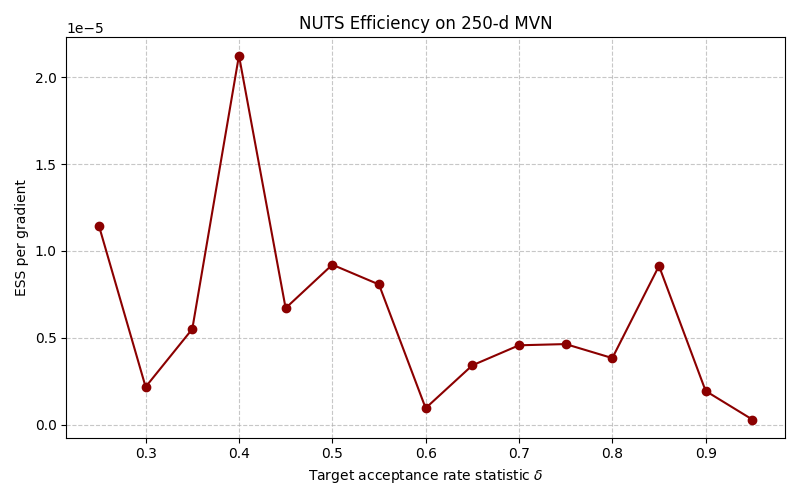
\includegraphics[width=0.85\textwidth]{MVN/250d_efficiency_plot.png}
        \caption{ESS/gradient for NUTS vs.\ best-tuned HMC on a 250-D Gaussian with random Wishart precision matrix. NUTS matches or exceeds HMC by roughly a factor of two without trajectory-length tuning.}
    \end{figure}
\end{frame}

\begin{frame}{Benchmark 2: Bayesian Logistic Regression (25-D)}
    \begin{figure}
        \centering
        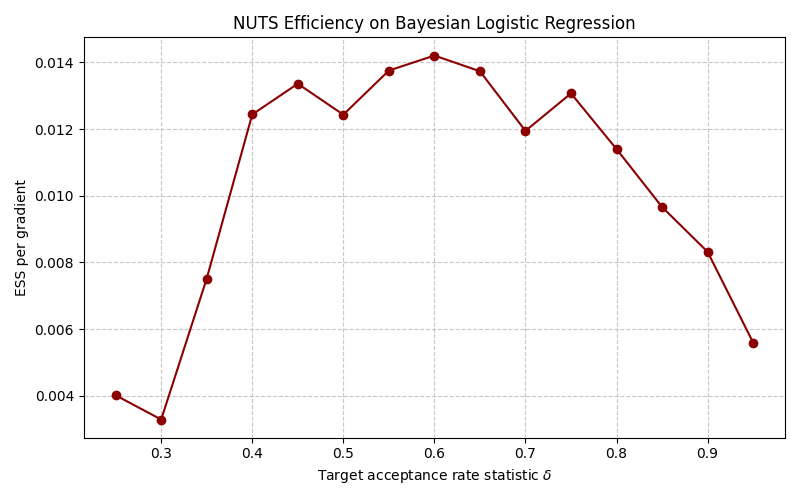
\includegraphics[width=0.85\textwidth]{LR/LR_efficiency_plot.png}
        \caption{ESS/gradient on Bayesian Logistic Regression fitted to the German Credit dataset (25 parameters). NUTS achieves comparable efficiency to the best-tuned HMC.}
    \end{figure}
\end{frame}

\begin{frame}{Benchmark 3: Stochastic Volatility (3001-D)}
    \begin{figure}
        \centering
        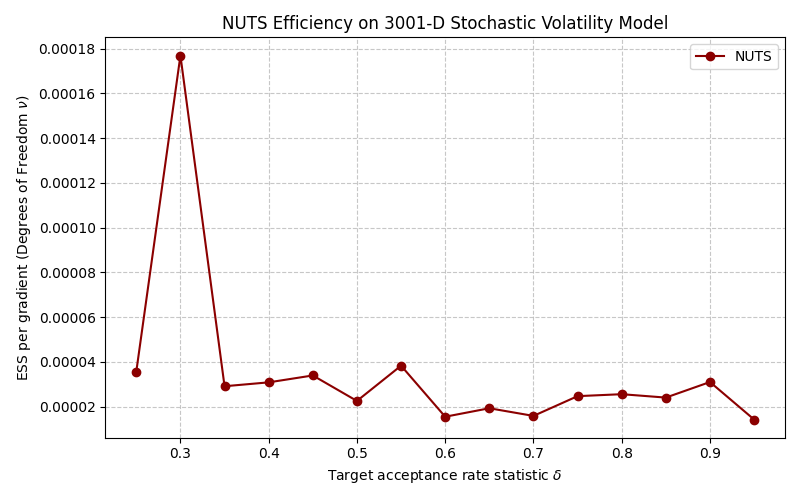
\includegraphics[width=0.85\textwidth]{SV/SV_efficiency_plot.png}
        \caption{ESS/gradient on the Stochastic Volatility model fitted to S\&P~500 returns (3001-D). NUTS outperforms HMC by roughly a factor of 1.5 without requiring any tuning.}
    \end{figure}
\end{frame}

\begin{frame}{Dual Averaging Convergence}
    \vspace*{-0.25cm}
    \begin{figure}
        \centering
        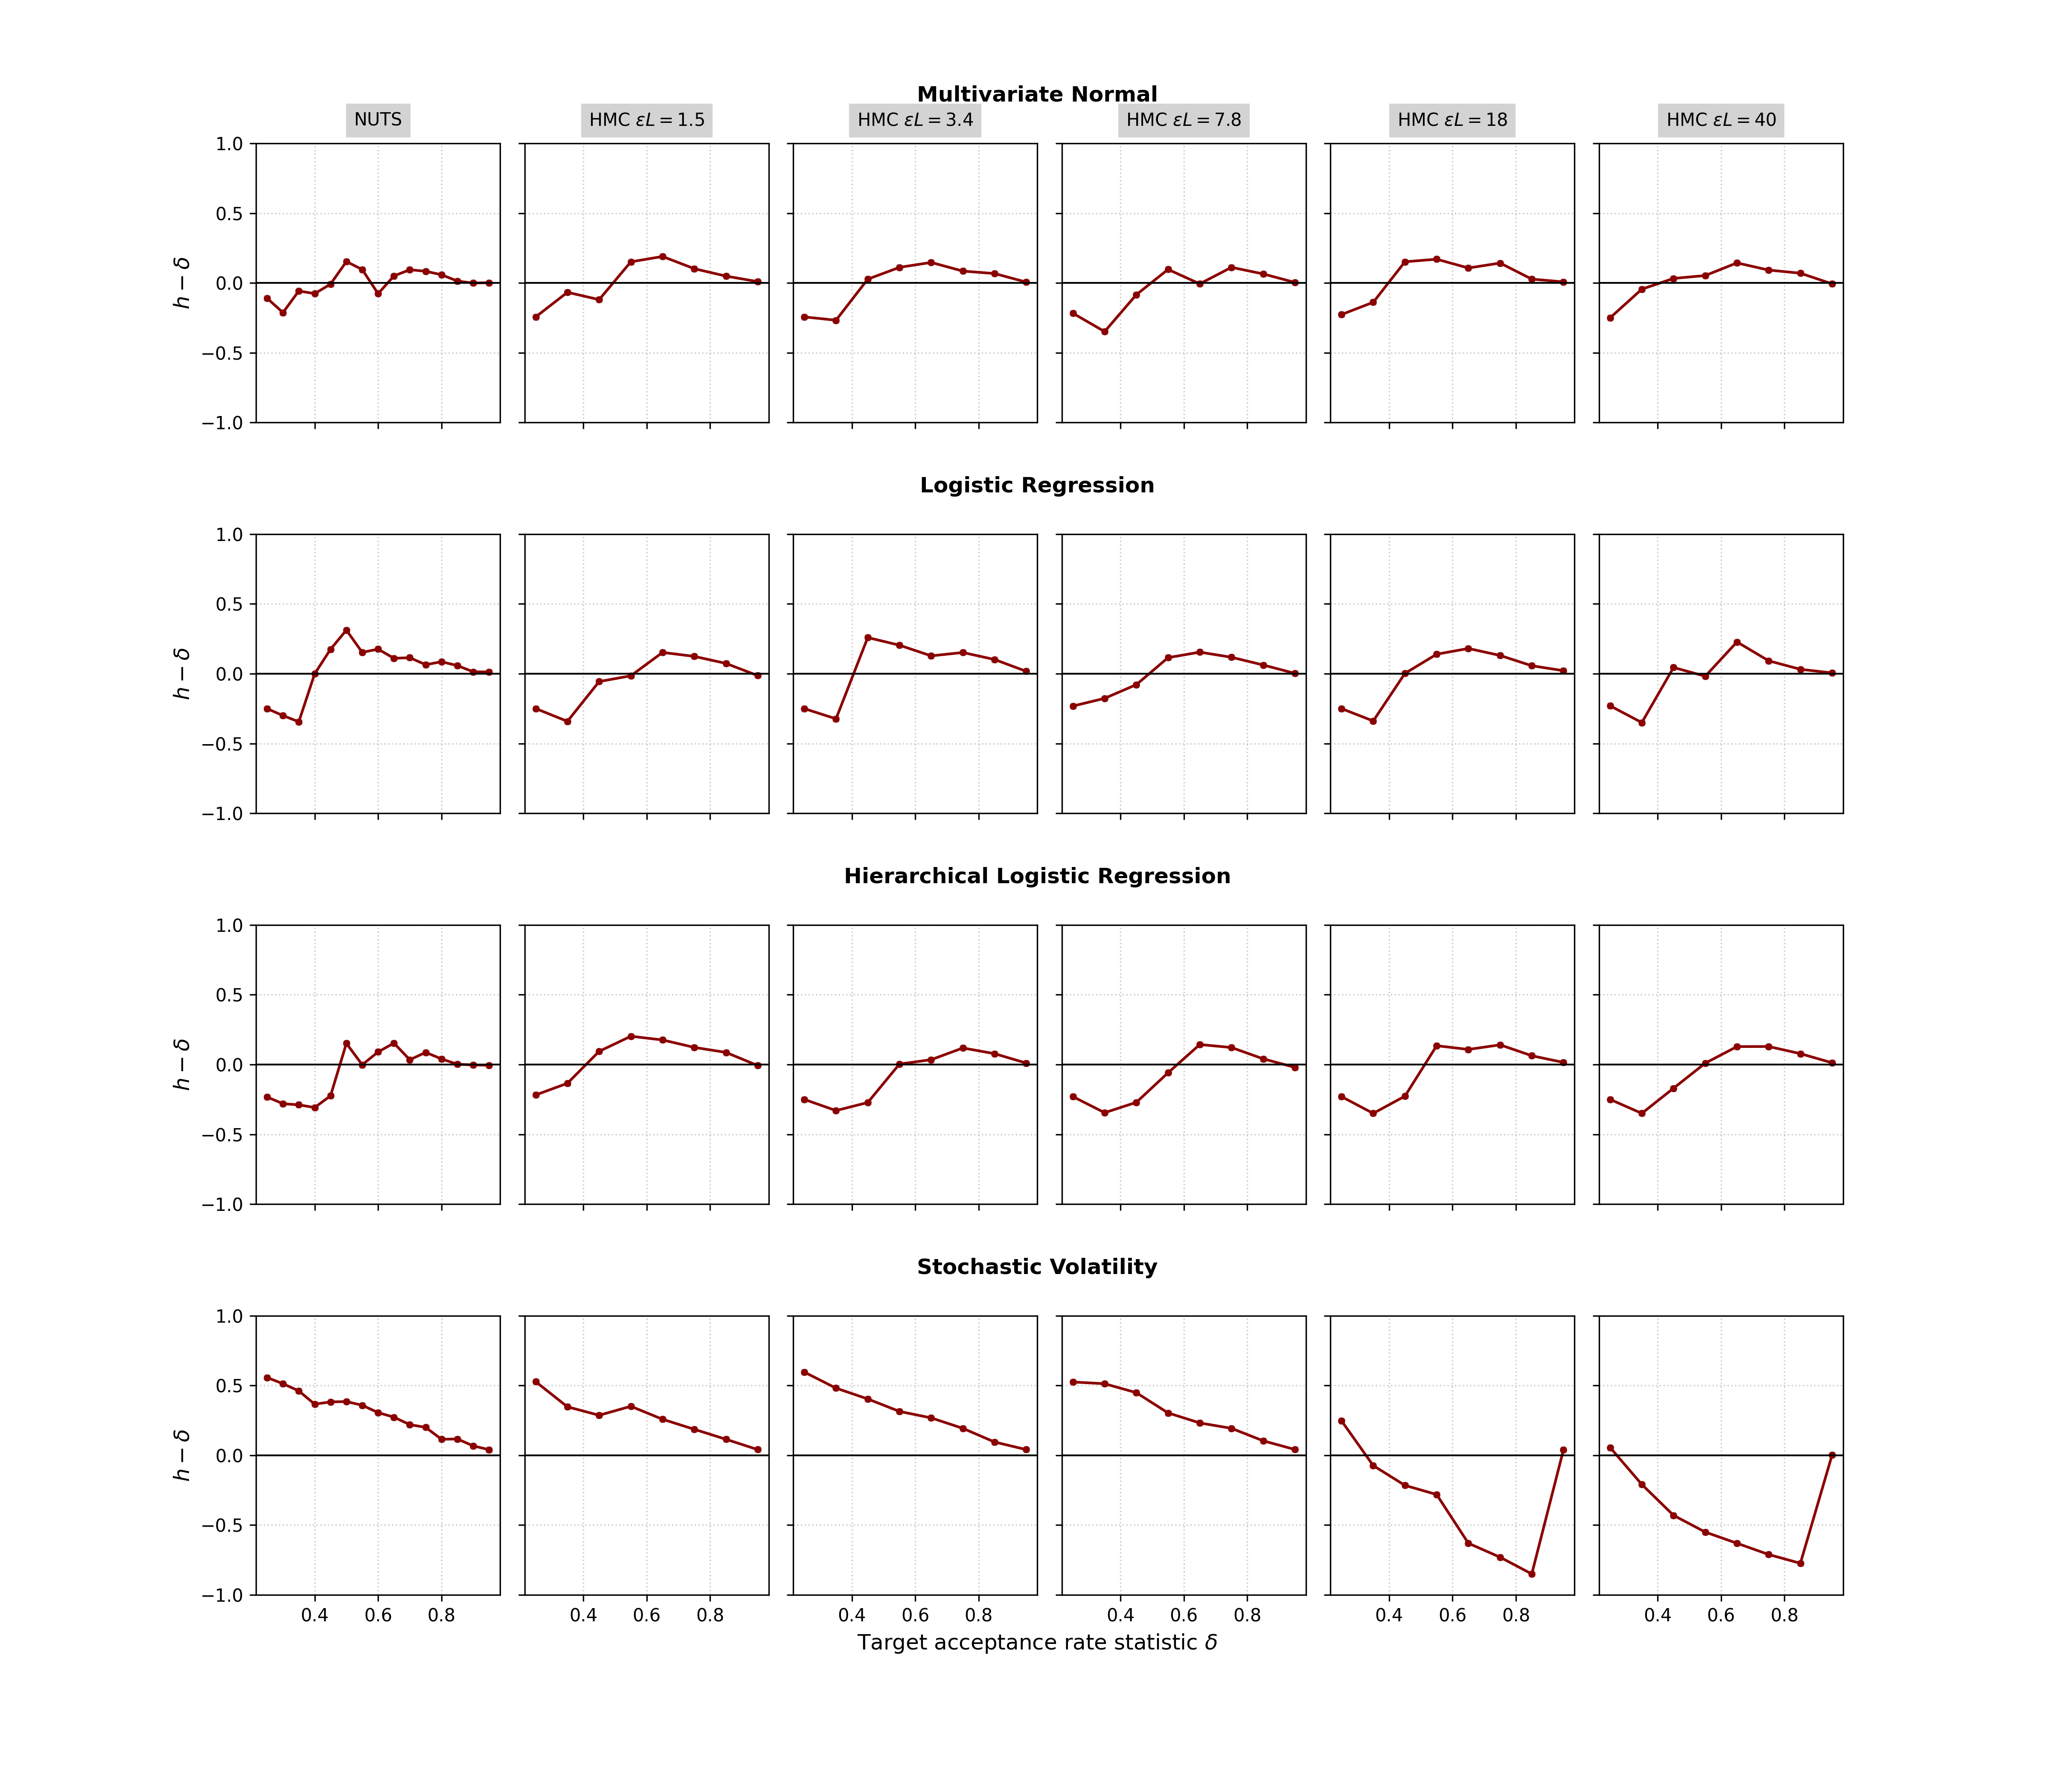
\includegraphics[width=0.78\textwidth]{discrepancies_plot.png}
        \vspace*{-0.7cm}
        \caption{Discrepancy plots ($h - \delta$ across $\delta$) for all four original benchmarks. The dual-averaging scheme reliably drives the acceptance statistic towards the target $\delta$ within a few hundred warm-up iterations.}
    \end{figure}
\end{frame}


% ==============================================================================
% SECTION 5: BEYOND THE PAPER --- STRESS TESTS
% ==============================================================================
%\section{Beyond the Paper: Stress Tests}

\begin{frame}{Motivation}
    The original evaluation is limited to \textbf{unimodal or mildly structured} targets.

    \vspace{0.3cm}
    We design three experiments targeting pathologies common in modern Bayesian models:
    \begin{enumerate}
        \item \textbf{Extreme multimodality} --- Bayesian Neural Network
        \item \textbf{Dense correlations} --- Gaussian Process Classification
        \item \textbf{Spatially varying geometry} --- Neal's Funnel
    \end{enumerate}

    \vspace{0.3cm}
    These stress tests probe failure modes of HMC that are \textbf{unexplored in the original paper}.
\end{frame}

% --- Stress Test 1: BNN ---

\begin{frame}{Stress Test 1: Bayesian Neural Network (191-D)}
    \textbf{Setup:}
    \begin{itemize}
        \item Two-hidden-layer BNN ($30 \to 5 \to 5 \to 1$), 191 parameters
        \item $\mathcal{N}(0, 100)$ priors on all weights and biases
        \item UCI Breast Cancer dataset
        \item Weight-permutation symmetries create $5! \times 5! = 14{,}400$ equivalent modes
    \end{itemize}

    \vspace{0.3cm}
    \textbf{Configuration:} $\delta = 0.65$, $M = 300$, $M_{\text{adapt}} = 150$

    \vspace{0.2cm}
    NUTS adapts trajectory lengths between 1 and 64 leapfrog steps, traversing curved valleys connecting symmetric modes. HMC, constrained to a fixed trajectory, overshoots or undershoots and stalls in a single mode.
\end{frame}

\begin{frame}{BNN: Trajectory Lengths and Efficiency}
    \begin{figure}
        \centering
        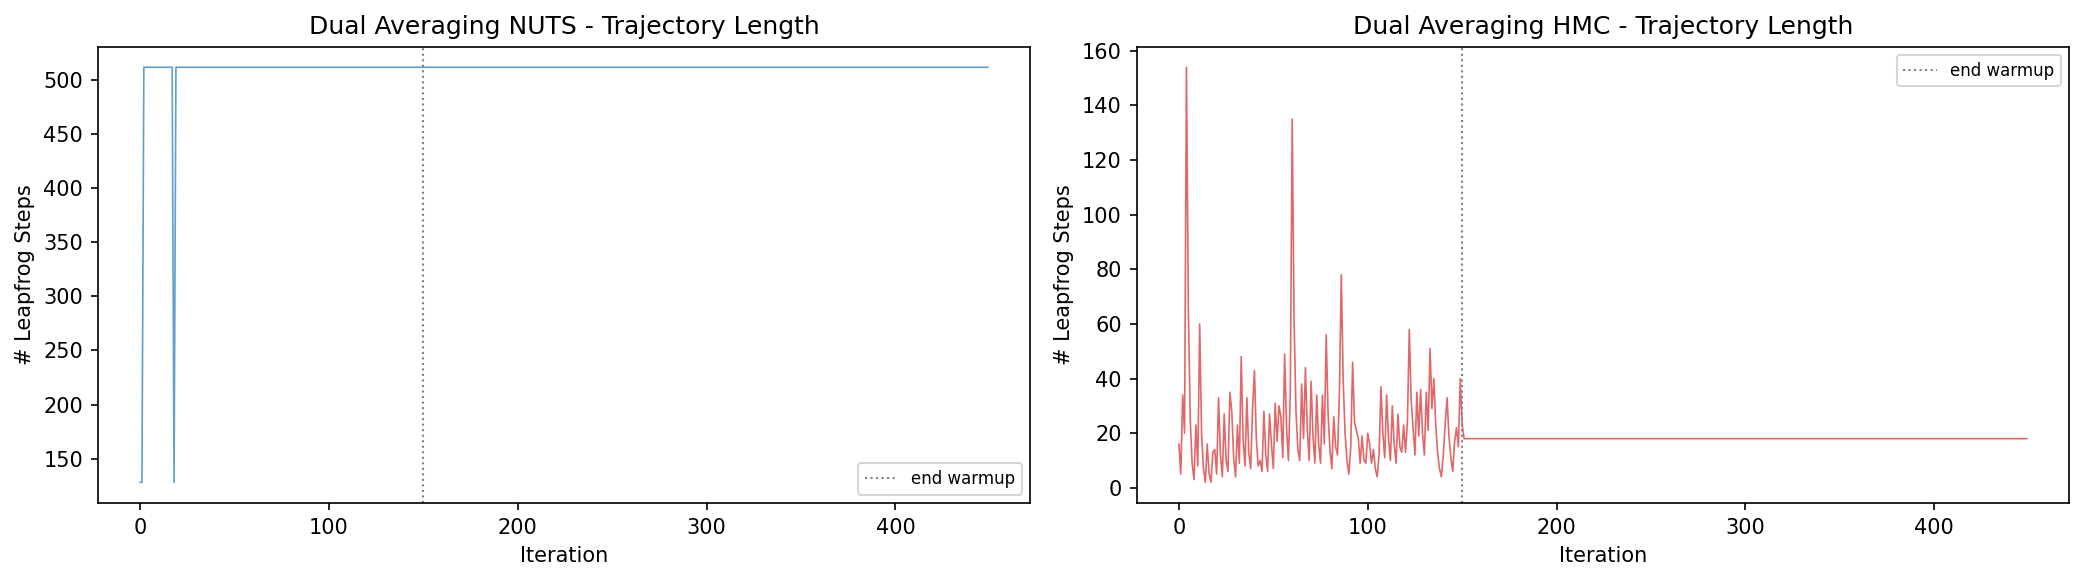
\includegraphics[width=\textwidth]{BNN/trajectory_lengths.png}
        \caption{NUTS trajectory lengths on the BNN posterior. Lengths concentrate on powers of two, confirming the U-turn criterion triggers at complete doublings. The adaptive mechanism is essential for navigating the multimodal landscape.}
    \end{figure}
\end{frame}

\begin{frame}{BNN: Trace Plots}
    \vspace*{-0.25cm}
    \begin{figure}
        \centering
        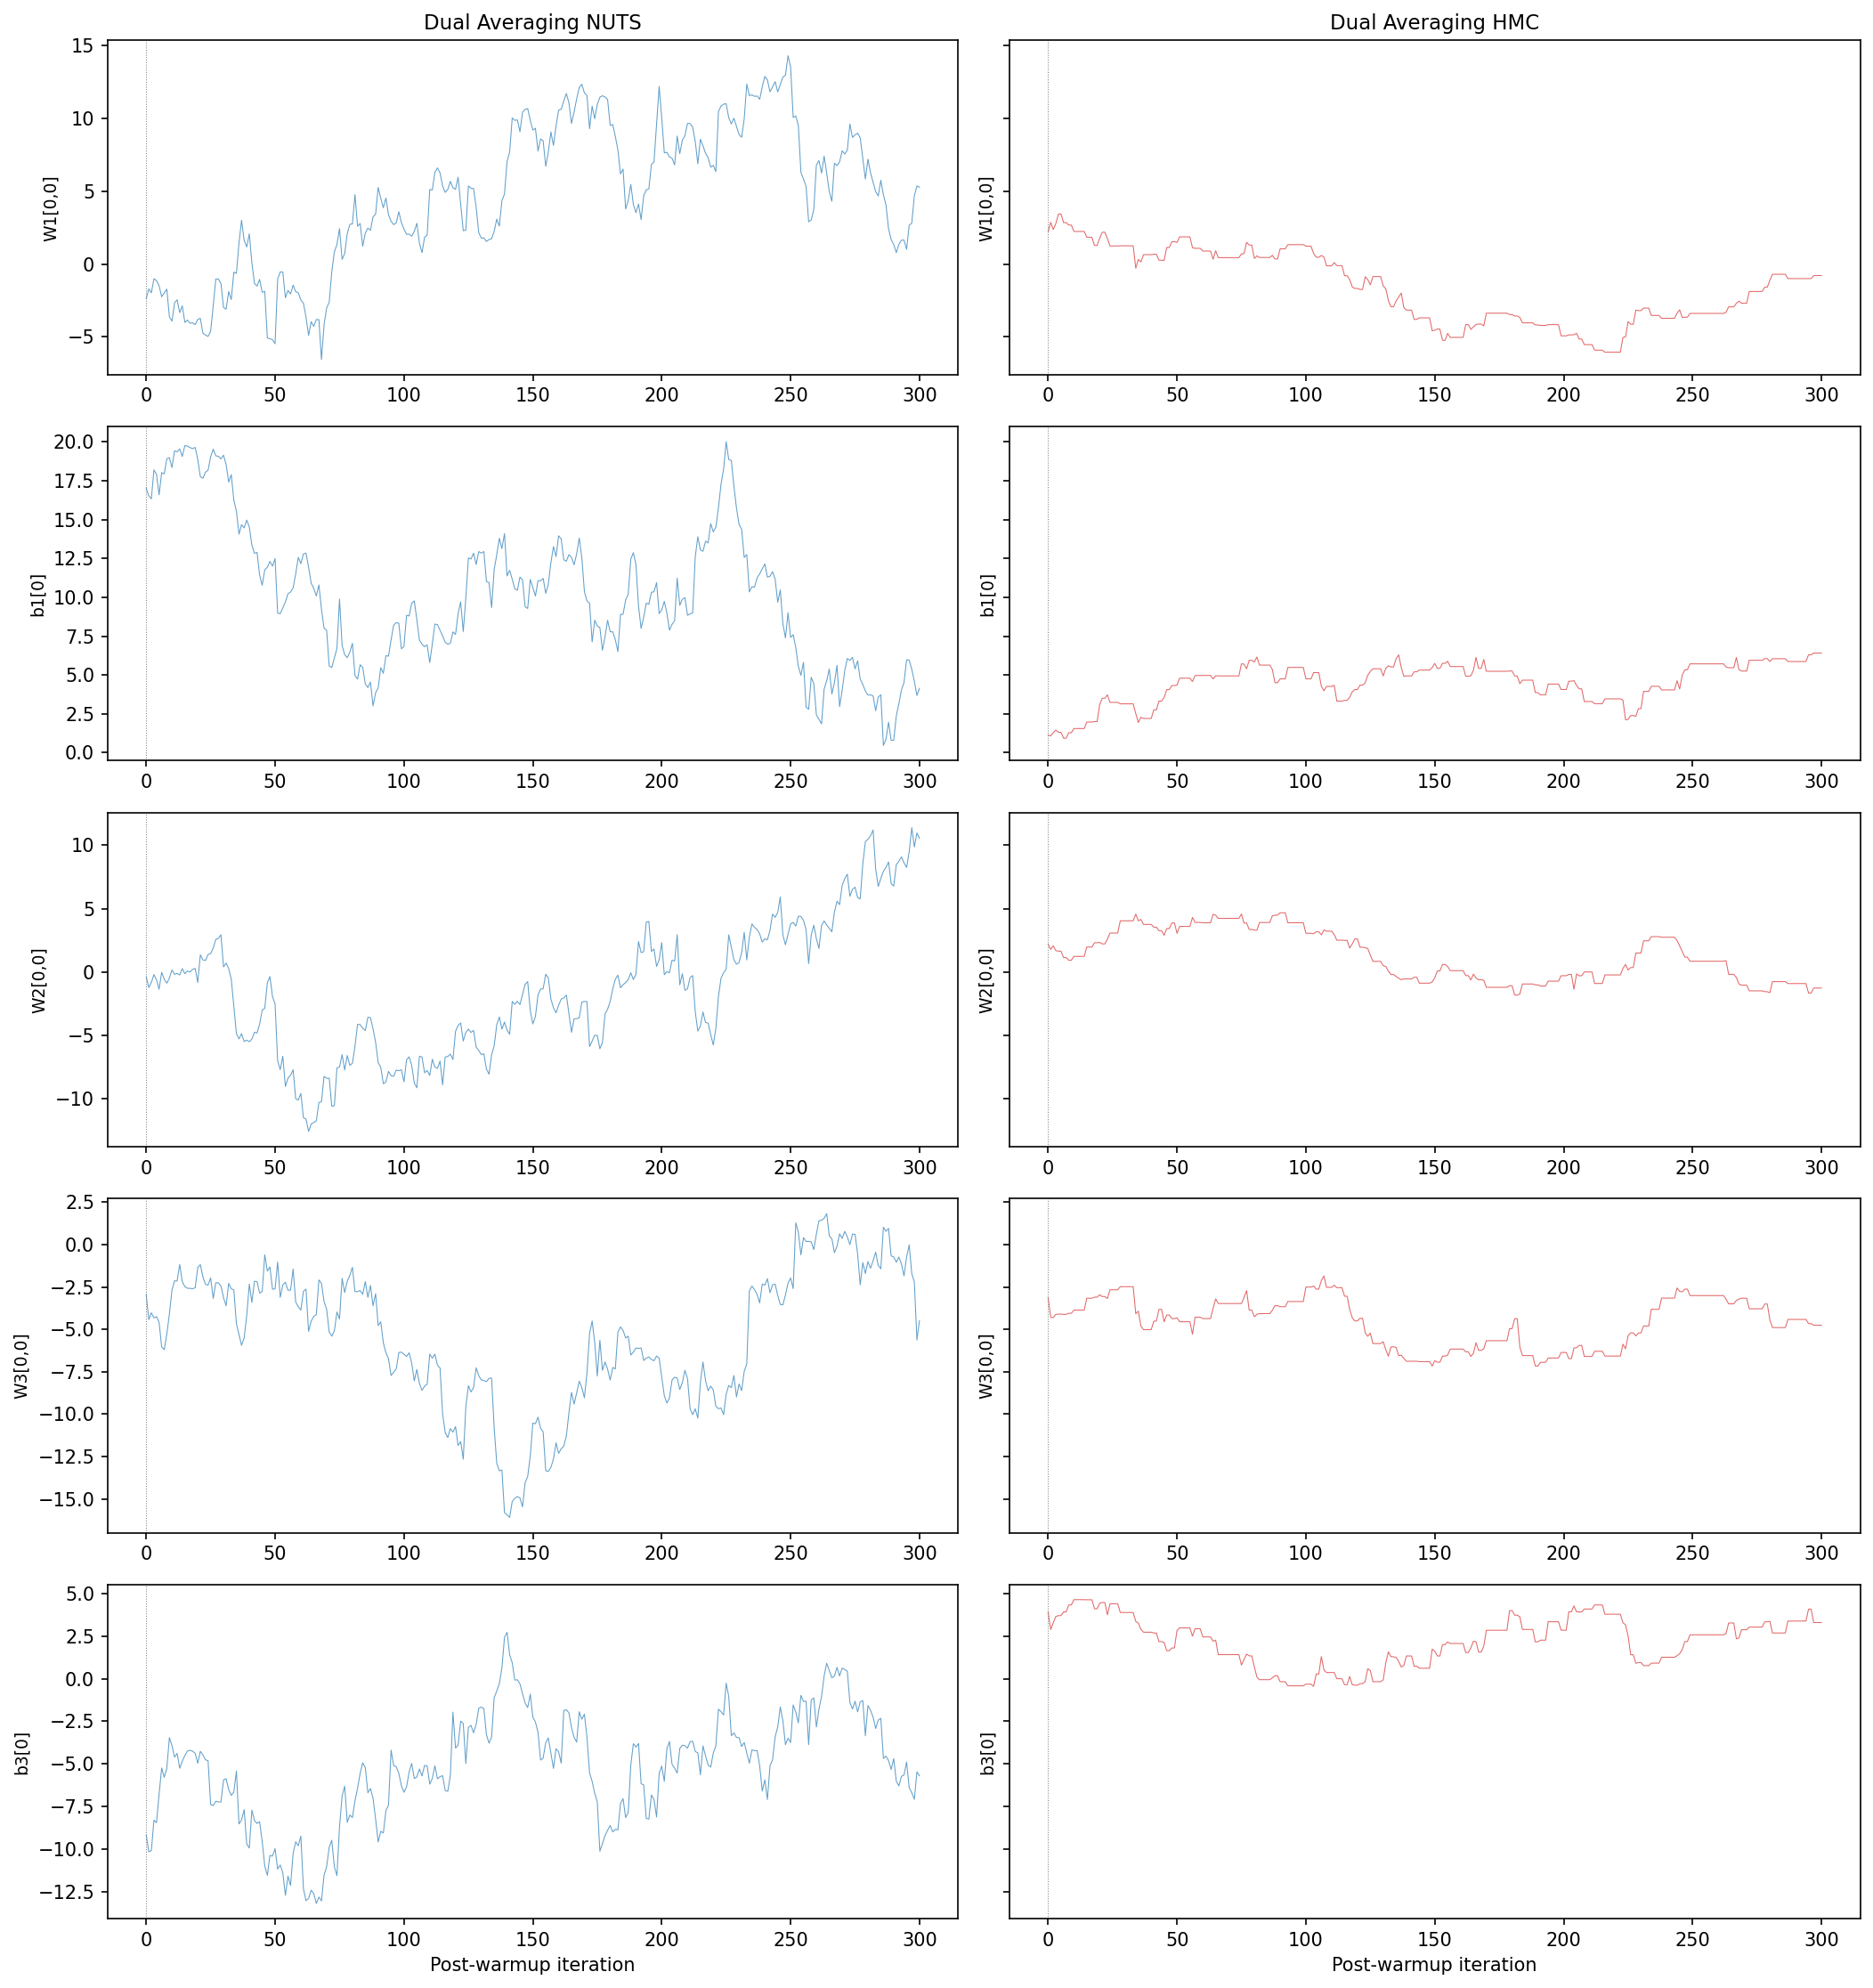
\includegraphics[width=0.6\textwidth]{BNN/trace_plots.png}
        \vspace*{-0.2cm}
        \caption{Trace plots on the BNN posterior. NUTS explores a wider range of weight values, while HMC exhibits prolonged stagnation in a single mode.}
    \end{figure}
\end{frame}

\begin{frame}{BNN: Efficiency Comparison}
    \begin{figure}
        \centering
        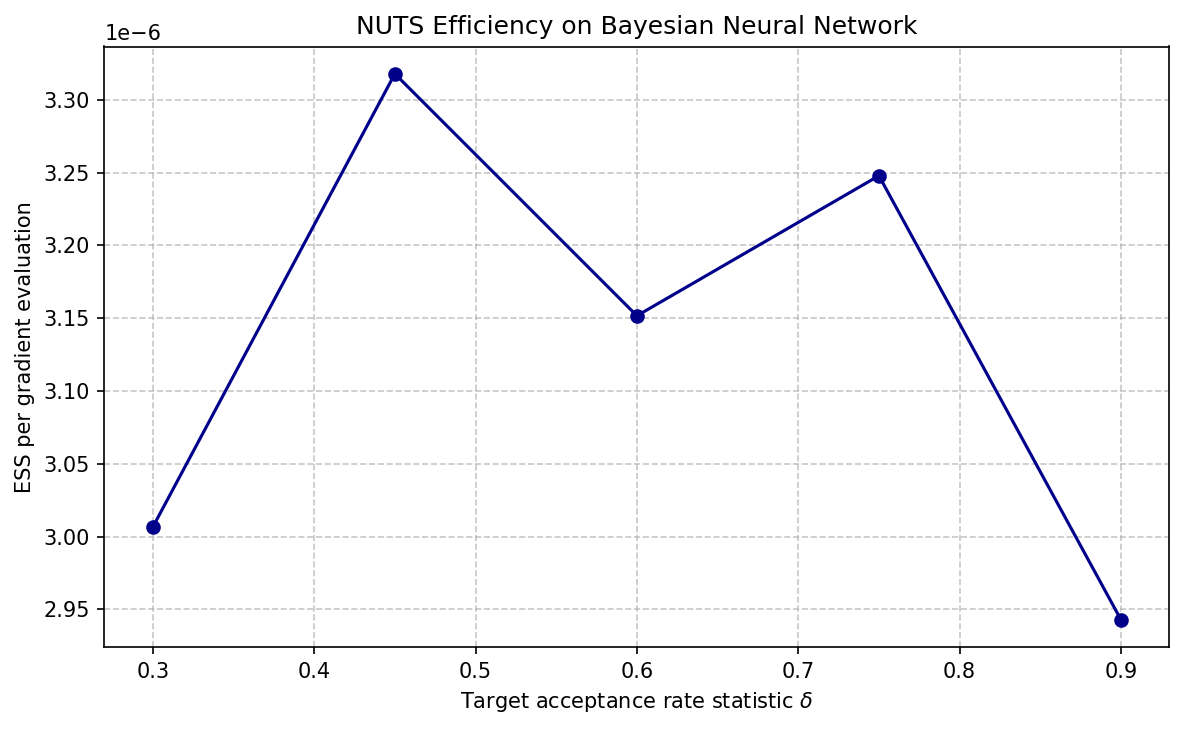
\includegraphics[width=0.85\textwidth]{BNN/BNN_efficiency_plot.png}
        \caption{ESS/gradient comparison on the BNN. NUTS achieves higher effective samples per gradient evaluation than HMC across all tested configurations.}
    \end{figure}
\end{frame}

% --- Stress Test 2: GPC ---

\begin{frame}{Stress Test 2: GP Classification (150-D)}
    \textbf{Setup:}
    \begin{itemize}
        \item GP classification with RBF kernel ($\ell = 1$, $\sigma_f^2 = 1$)
        \item 150 points from the California Housing dataset
        \item Fully dense $150 \times 150$ covariance matrix $K$
        \item Gradient $\nabla\!\log p(f) = -K^{-1}f + y \odot \sigma(-y \odot f)$ requires a dense solve at every leapfrog step
    \end{itemize}

    \vspace{0.3cm}
    \textbf{Configuration:} $M = 500$, $M_{\text{adapt}} = 250$

    \vspace{0.2cm}
    NUTS achieves $2.5 \times 10^{-3}$ ESS/grad at $\delta = 0.7$, requiring fewer gradient evaluations than HMC for equivalent effective samples.
\end{frame}

\begin{frame}{GPC: Kernel Matrix and Posterior Correlations}
    \vspace*{-0.25cm}
    \begin{figure}
                \centering
                \includegraphics[width=0.75\textwidth]{GPC/kernel_matrix.png}
                \vspace*{-0.2cm}
                \caption{RBF kernel matrix $K$ exhibiting dense correlation structure.}
            \end{figure}
        \vspace*{-0.3cm}
            \begin{figure}
                \centering
                \includegraphics[width=0.75\textwidth]{GPC/posterior_correlations.png}
                \vspace*{-0.2cm}
                \caption{Posterior correlations among the latent function values $f$.}
            \end{figure}

\end{frame}

\begin{frame}{GPC: Trajectory Lengths and Efficiency}
    \begin{figure}
        \centering
        
\includegraphics[width=\textwidth]{GPC/trajectory_lengths.png}
        \caption{NUTS trajectory lengths on the GP classification posterior. The dense correlation structure demands longer trajectories to traverse the strongly coupled latent space.}
    \end{figure}
\end{frame}

\begin{frame}{GPC: Efficiency Comparison}
    \begin{figure}
        \centering
        \includegraphics[width=0.85\textwidth]{GPC/GPC_efficiency_plot.png}
        \caption{ESS/gradient on GP classification. NUTS requires fewer gradient evaluations than HMC for equivalent effective samples under dense correlations.}
    \end{figure}
\end{frame}

% --- Stress Test 3: Neal's Funnel ---

\begin{frame}{Stress Test 3: Neal's Funnel (10-D)}
    \textbf{Model:}
    \[
        v \sim \mathcal{N}(0, 9), \qquad x_i \mid v \sim \mathcal{N}(0, e^v), \quad i = 1, \dots, 9
    \]

    \vspace{0.2cm}
    \textbf{Challenge:}
    \begin{itemize}
        \item As $v \to -\infty$: conditional variance $e^v \to 0$ creates a microscopic neck demanding tiny steps
        \item Wide top ($v > 0$) requires large steps
        \item HMC's fixed step size cannot handle both regimes simultaneously
    \end{itemize}

    \vspace{0.3cm}
    This is a canonical pathological target \cite{neal2003slice} that exposes the limitations of fixed-trajectory samplers.
\end{frame}

\begin{frame}{Funnel: Scatter Plots}
    \vspace*{-0.25cm}
    \begin{figure}
        \centering
        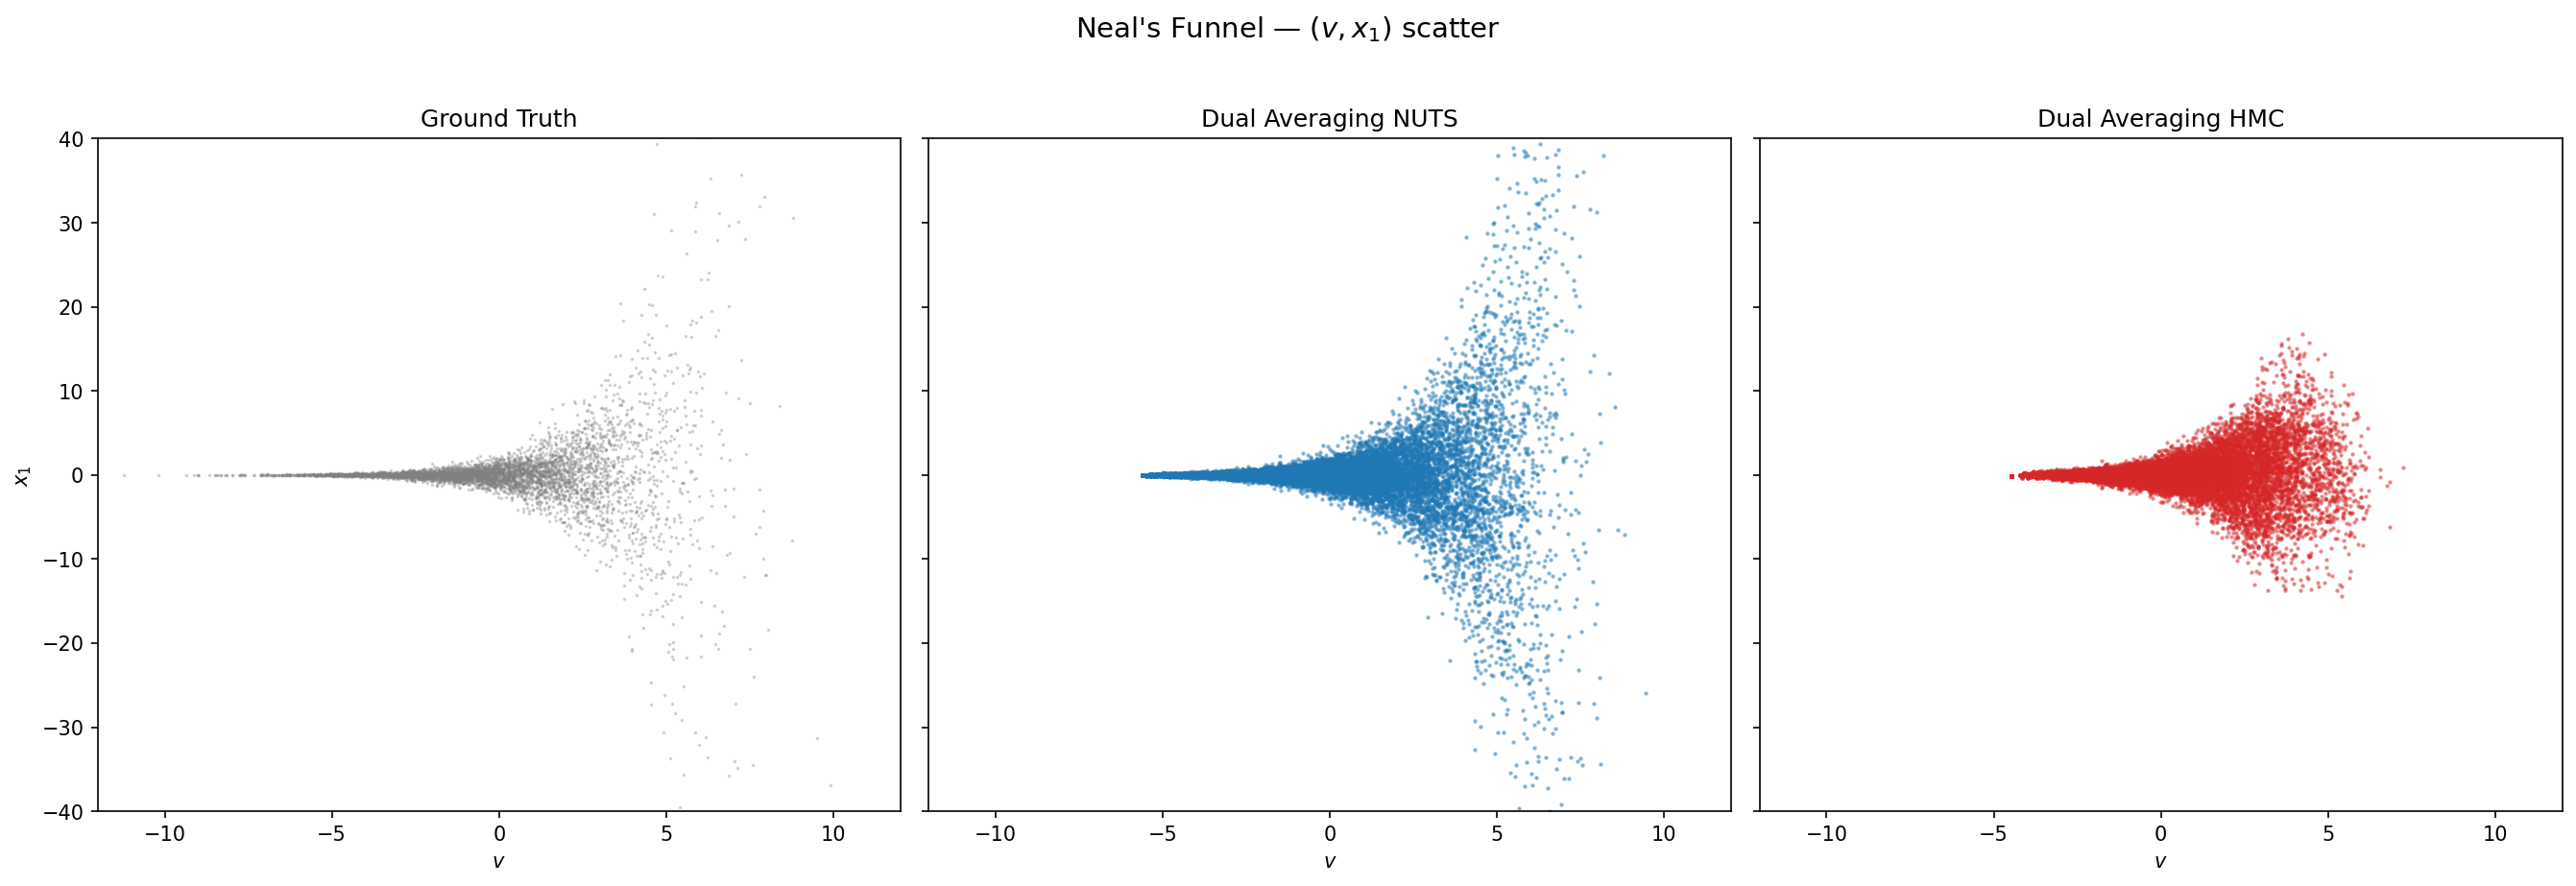
\includegraphics[width=\textwidth]{Funnel/funnel_scatter.png}
        \caption{Neal's Funnel $(v, x_1)$ scatter. \textbf{Left:} ground truth. \textbf{Centre:} NUTS covers the full funnel. \textbf{Right:} HMC fails to enter the narrow neck ($v < 0$), producing biased samples.}
    \end{figure}
\end{frame}

\begin{frame}{Funnel: Trace Plots}
    \begin{figure}
        \centering
        
\includegraphics[width=0.7\textwidth]{Funnel/trace_plots.png}
        \vspace*{-0.2cm}
        \caption{Trace plots on Neal's Funnel. NUTS transitions freely across the full $v$ range with good mixing. HMC gets trapped with flat segments indicating rejected proposals.}
    \end{figure}
\end{frame}

\begin{frame}{Funnel: Marginal Distribution of $v$}
    \begin{figure}
        \centering
        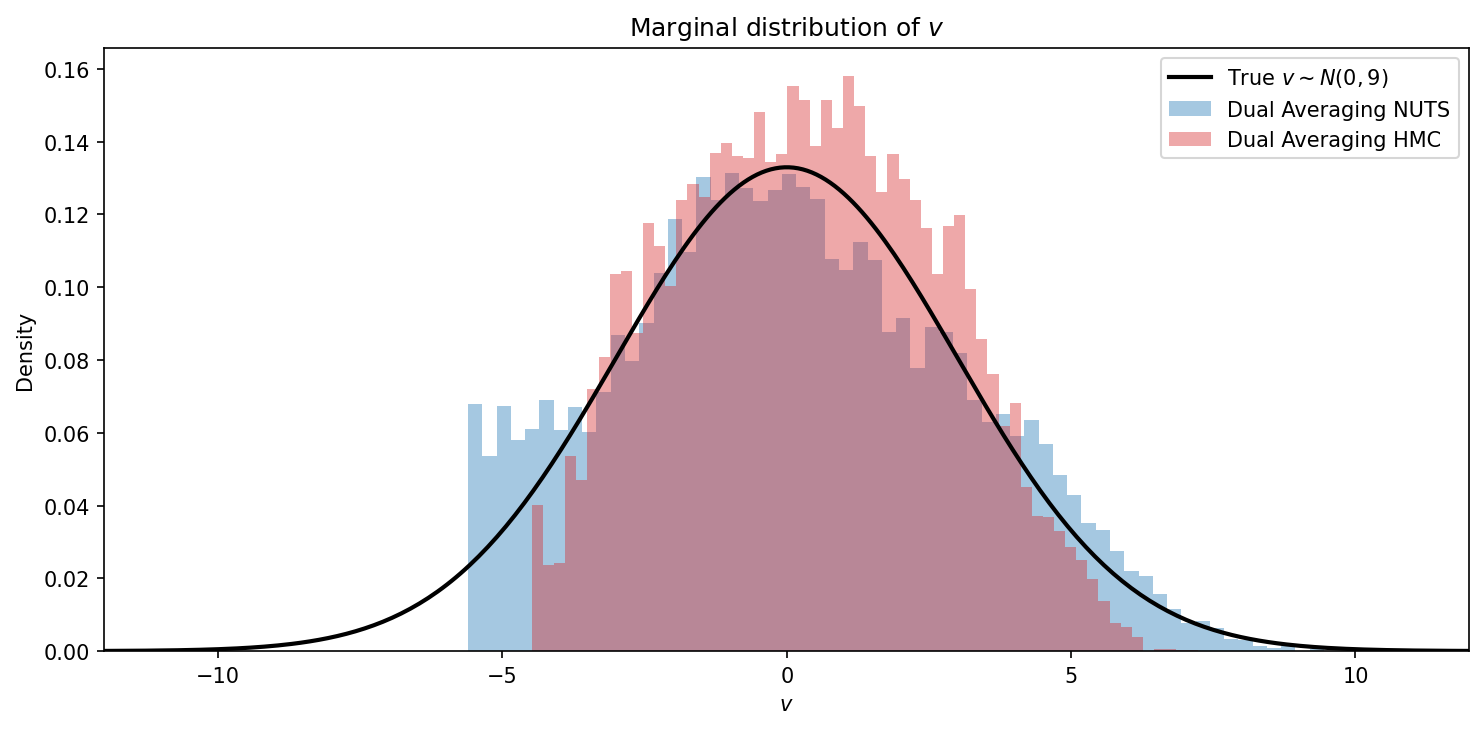
\includegraphics[width=0.85\textwidth]{Funnel/v_marginal.png}
        \caption{Marginal distribution of $v$. NUTS recovers $\mathrm{Var}(v) \approx 9$ (the true value), while HMC severely underestimates it, confined to $v \in [0, 4]$.}
    \end{figure}
\end{frame}

\begin{frame}{Funnel: Efficiency Comparison}
    \begin{figure}
        \centering
        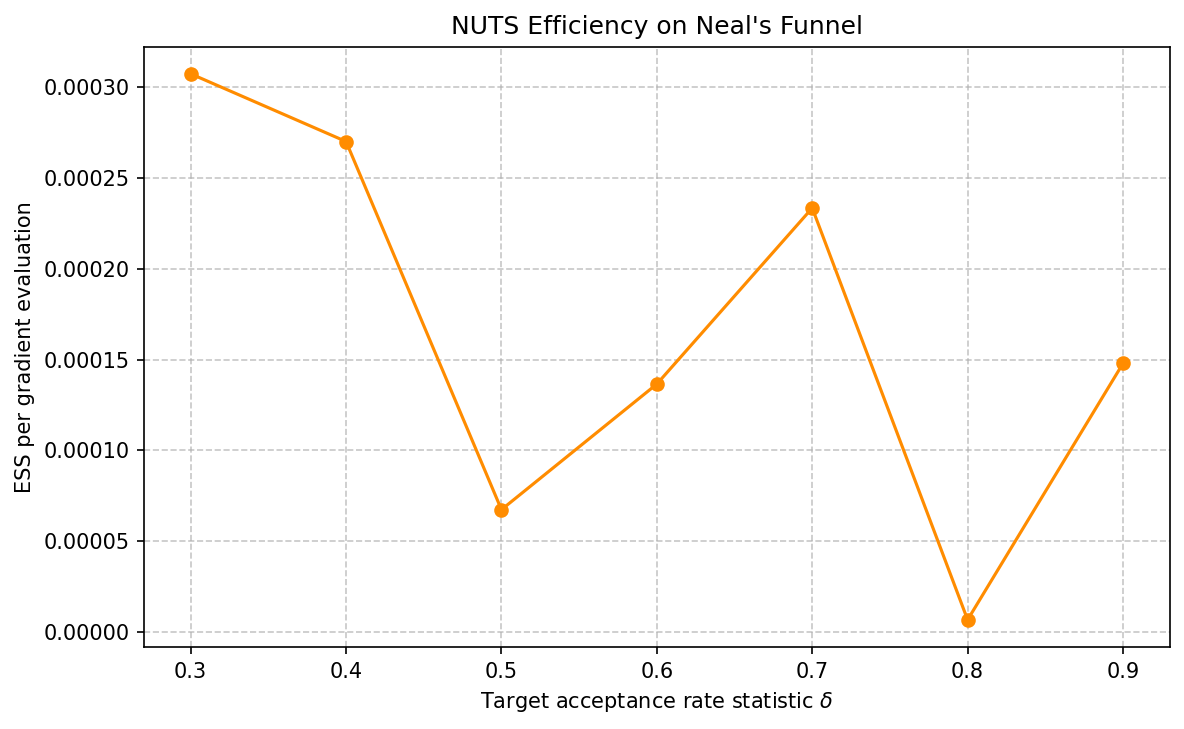
\includegraphics[width=0.85\textwidth]{Funnel/Funnel_efficiency_plot.png}
        \caption{ESS/gradient on Neal's Funnel. The gains are most dramatic when the posterior geometry varies spatially.}
    \end{figure}
\end{frame}


% ==============================================================================
% SECTION 6: CONCLUSION
% ==============================================================================
%\section{Conclusion}

\begin{frame}{Summary}
    \textbf{Strengths of the article:}
    \begin{itemize}
        \item Resolves a central practical limitation of HMC through a conceptually simple yet theoretically rigorous construction
        \item No-U-Turn criterion and recursive doubling preserve detailed balance
        \item Dual averaging for step-size adaptation makes NUTS essentially tuning-free
    \end{itemize}

    \vspace{0.3cm}
    \textbf{Limitations:}
    \begin{itemize}
        \item Dual-averaging hyperparameters justified empirically, not theoretically
        \item Performance guarantees are mainly asymptotic
        \item Original experiments cover a limited range of posterior geometries
    \end{itemize}
\end{frame}

\begin{frame}{Key Takeaways}
    \textbf{Our implementation validates} the original results: NUTS matches or exceeds the best-tuned HMC on all four benchmarks while eliminating trajectory-length tuning.

    \vspace{0.3cm}
    \textbf{Our stress tests} demonstrate that adaptive trajectory length is critical on posteriors with complex geometries:
    \begin{itemize}
        \item \textbf{BNN:} NUTS navigates 14,400 equivalent modes; HMC stagnates
        \item \textbf{GPC:} NUTS handles dense $150 \times 150$ correlations efficiently
        \item \textbf{Neal's Funnel:} NUTS covers the full funnel; HMC fails catastrophically
    \end{itemize}

    \vspace{0.3cm}
    NUTS is confirmed as a suitable \textbf{general-purpose inference engine} for modern Bayesian models.
\end{frame}


% ==============================================================================
% SECTION : BIBLIOGRAPHY
% ==============================================================================
%\section*{}
\begin{frame}[allowframebreaks]{Bibliography}
    \printbibliography[heading=none]
\end{frame}


% ==============================================================================
% SECTION : APPENDIX
% ==============================================================================
%\section*{Appendix}

\begin{frame}{Appendix: BNN Adaptation Diagnostics}
    \begin{figure}
        \centering
        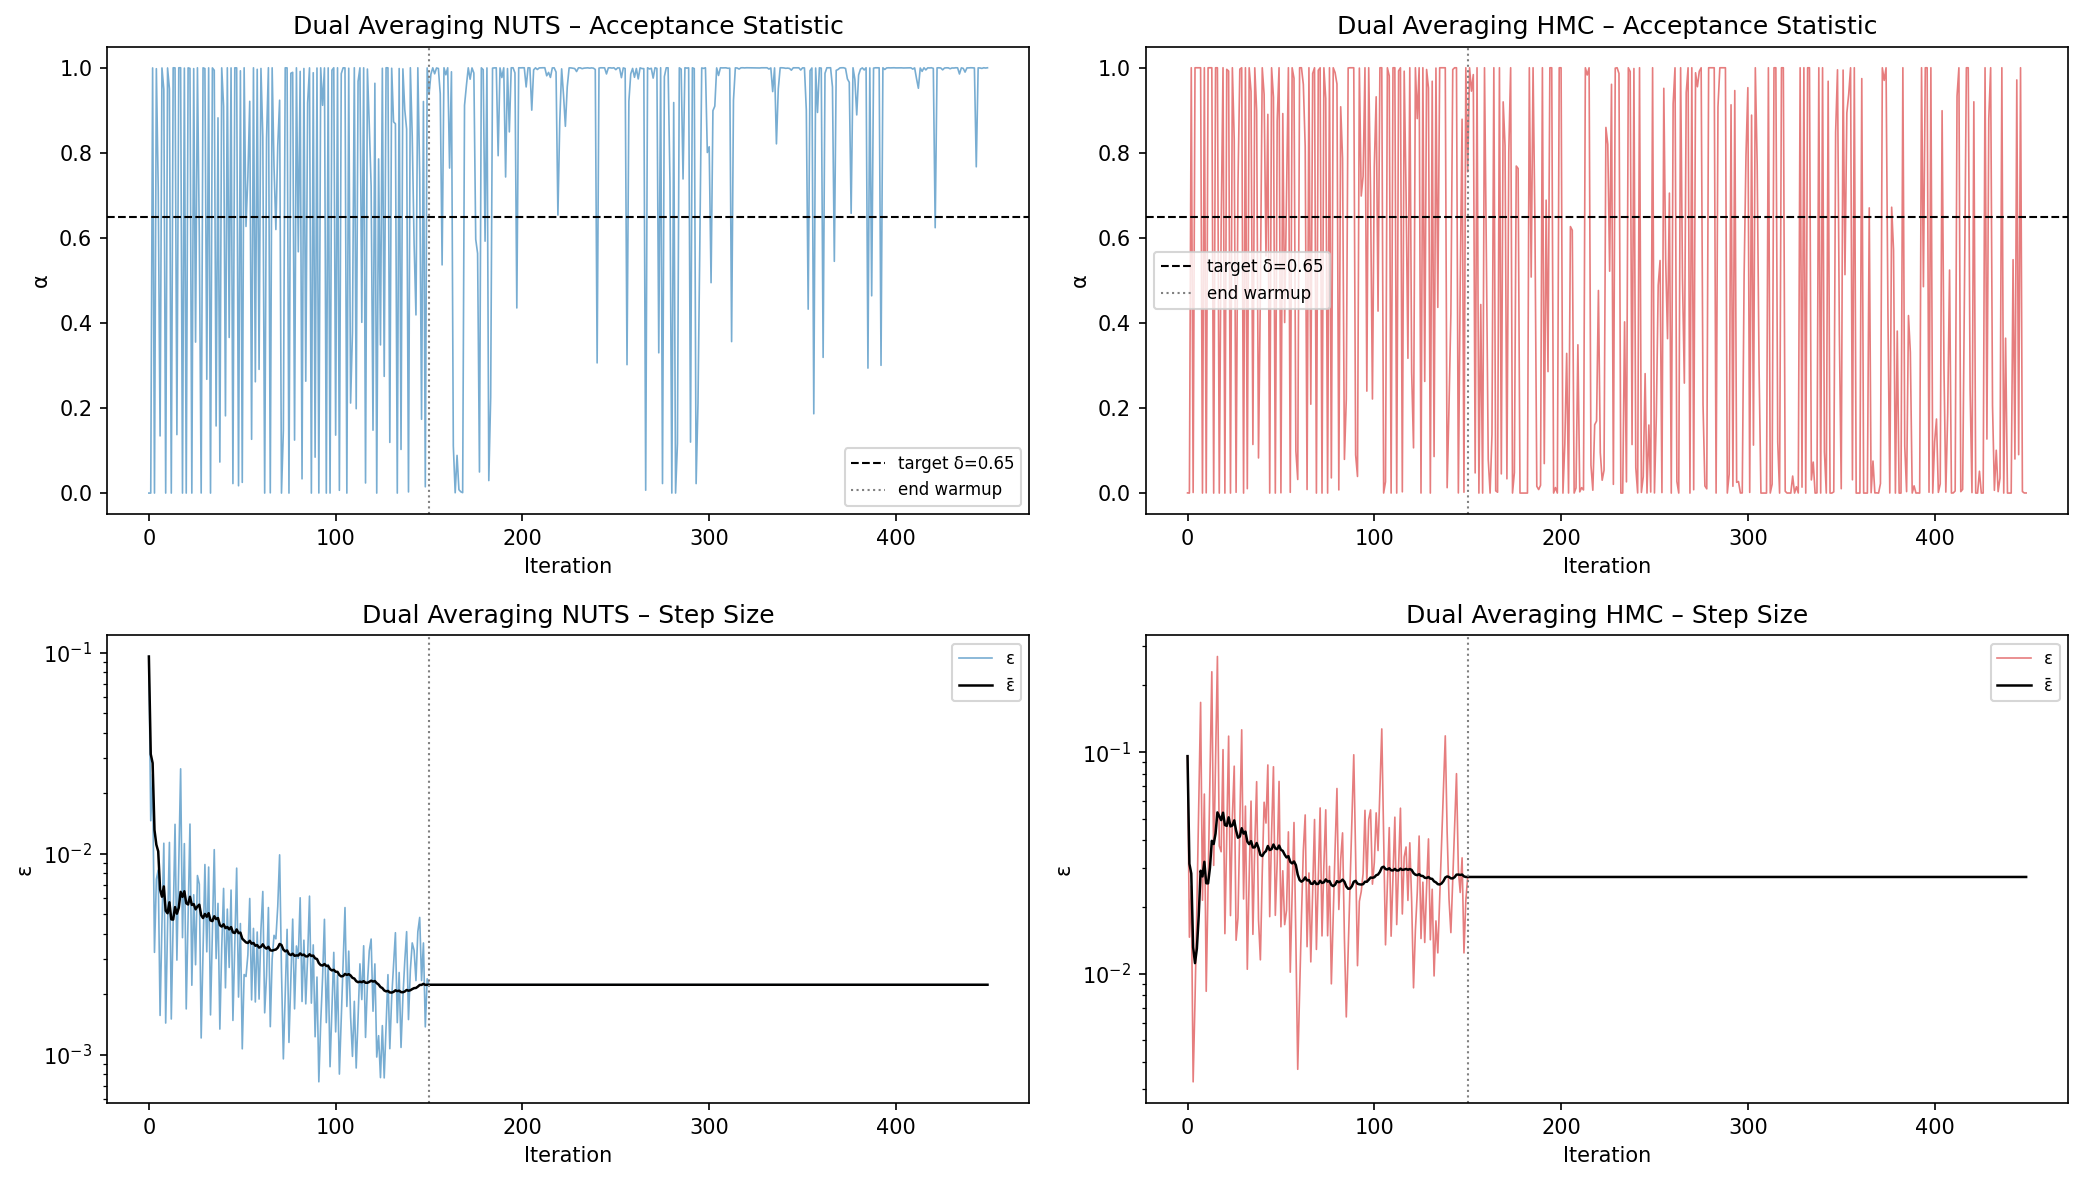
\includegraphics[width=\textwidth]{BNN/adaptation_diagnostics.png}
        \caption{Dual-averaging convergence on the BNN posterior. The step size $\bar{\varepsilon}$ stabilises within the warm-up phase.}
    \end{figure}
\end{frame}

\begin{frame}{Appendix: GPC Trace Plots}
    \vspace*{-0.25cm}
    \begin{figure}
        \centering
        
\includegraphics[width=0.6\textwidth]{GPC/trace_plots.png}
        \vspace*{-0.2cm}
        \caption{Trace plots for selected latent function values on the GP classification posterior.}
    \end{figure}
\end{frame}

\begin{frame}{Appendix: Funnel Trajectory Lengths}
    \begin{figure}
        \centering
        
\includegraphics[width=\textwidth]{Funnel/trajectory_lengths.png}
        \caption{NUTS trajectory lengths on Neal's Funnel. The adaptive mechanism adjusts trajectory length to the local geometry.}
    \end{figure}
\end{frame}


\end{document}